\chapter{Peierls-Hubbard model}
\label{chap:model}

% As mentioned earlier \ref{sec:scope}: 
% - Lattice inhomogeneities limit the applicability of $k$-space formalism.
% - Correlated electron-lattice motion prevents the use of Born-Openheimer approximation
% We propose a very simple but exact model that captures the polaronic behaviour of a CuO$_2$ cluster.
% This model has been successfully used to explain the O-Cu split distance in YBCO

% This chapter:
% - Describes the model hamiltonian
% - Describes a basis set
% - Presents two useful projections (phonon coordinates and electron occupation)

\section{Description}

The hamiltonian we used to describe two holes in the O(4)-Cu(1)-O(4) cluster with an electron-lattice correlated movement consists of three parts \cite{Salkola1994}:

\begin{equation}\label{eq:full-hamiltonian}
H = H_{el} + H_{ph} + H_{el-ph}
\end{equation}

\noindent corresponding to the electronic contribution, the phonon energies and the electron-phonon (lattice) coupling, respectively. 
The electron-phonon coupling term deviates this model from the Born-Oppenheimer (adiabatic) approximation and prevents the separation of hamiltionan eigenstates, $\Psi$, as products of purely electronic and phononic parts, $\Psi=\psi_{el}\psi_{ph}$, unless $H_{el-ph}=0$.
Nonetheless, as it will be discussed in section \ref{sec:classification}, even for coupling values greater than zero the hamiltonian eigenstates can be interpreted as mainly \textit{electronic} or \textit{phononic} in nature.

The electronic part is modeled as a single band Hubbard model for three sites with two holes in it. 
We denote $n_{i\sigma}=c_{i\sigma}^\dagger c_{i\sigma}$ as the hole-number operator with $c_{i\sigma}^\dagger$ creating a hole with spin $\sigma = \uparrow, \downarrow$ and $c_{i\sigma}$ destroying it; the site index $i=1,2,3$ indicates the two oxygen sites when  $i=1,3$ and the only copper site when $i=2$. 
The site energies are parametrized with $E_1=E_3=-E_2 \equiv E_0$. 
$U$ is the on-site Coulomb interaction and $t$ is the hopping energy between two adjacent sites. 
With these definitions, the electronic contribution is written as follows,

\begin{equation}\label{eq:electronic-part}
H_{el} = \sum_{\sigma,i=1}^3 E_i n_{\sigma i} + U\sum_{i=1}^3 n_{i\downarrow}n_{i\uparrow} + t\sum_{\sigma}(c_{1\sigma}^\dagger c_{2\sigma} + c_{2\sigma}^\dagger c_{3\sigma} + H.c.)
\end{equation}

For the lattice  part of the Hamiltonian, $H_{ph}$, we consider both symmetric (Raman) and antisymmetric (infrared) modes described by boson operators $b_R$ and $b_{ir}$ and bare frequencies $\omega_R$ and $\omega_{ir}$ respectively,
 
\begin{equation}\label{eq:phonon-part}
H_{ph} = \hbar \omega_{ir}b_{ir}^\dagger b_{ir} + \hbar \omega_R b_R^\dagger b_R
\end{equation}

% Figure with the two vibrational modes
 
The electron-lattice coupling term, $H_{el-ph}$ is introduced through the change in interatomic distances generated by Coulomb repulsion between different sites coupled with the Raman and infrared phonon modes\footnote{This term is written slightly different in \cite{MustredeLeon1992} however, both versions can be related noticing that $3 (n_1+n_3-4/3)=n_1-2n_2+n_3$.},
 
\begin{equation}\label{eq:coupling-part}
H_{el-ph} = \lambda_{ir}(b_{ir} + b_{ir}^\dagger)(n_3 - n_1) + \lambda_R (b_R + b_R^\dagger)(n_1 + n_3-s_0)
\end{equation}

Here $s_0$ is a constant used to avoid artificial shrinking of the cluster. 
For consistency with other works \cite{MustredeLeon1992,DeLeon1999,Leon2008,MirandaMena2007} we fix $s_0=4/3$.

% Describe how the different values for n_1, n_2, n_3 couple to phonons. Maybe include a figure here.

\section{Basis set}
\label{sec:basis-set}

The basis is $\ket{e_1,e_2,i,R}$ with $e_k$ being the position of the $k$-th hole ($e_i=1,2,3$), $i$ the number of \textit{infrared} phonons and $R$ the number of \textit{Raman} phonons. 
Formally, $i$ and $R$ should extend to infinity but the system converges to a stable behaviour (for the lower excitations) after considering just a few phonons. 
Our tests show that 30 phonons of each kind are enough to stabilize our results\footnote{There is another numerical instability present in the calculation of the isotopic shift of the first excitation (see section \ref{sec:polaron-isotopic-shift}) but this seems to be due to floating point errors in the calculations since all numbers are very close to zero.}

To build the hamiltonian we use a definite electron-ocuppation basis with the following labelling for each of the possible electron occupations:

\begin{equation}\label{eq:basis-set}\begin{array}{cccc}
1= & \uparrow \downarrow & - & - \\
2= & \uparrow & \downarrow & - \\
3= & \uparrow & - & \downarrow \\
4= & \downarrow & \uparrow & - \\
5= & - & \uparrow \downarrow & - \\
6= & - & \uparrow & \downarrow \\
7= & \downarrow & - & \uparrow \\
8= & - & \downarrow & \uparrow \\
9= & - & - & \uparrow \downarrow \end{array}\end{equation}


\section{Electronic part}

The electronic part $H_{el}$ is a 9x9 matrix

\begin{equation}\label{eq:electronic-matrix}
\left( \begin{array}{ccccccccc} 
U+2\epsilon &\;\;t\;\;&\;\;0\;\;&\;\;t\;\;&0&\;\;0\;\;&\;\;0\;\;&\;\;0\;\;&0 \\
t&0&t&0&t&0&0&0&0 \\
0&t&2\epsilon &0&0&t&0&0&0 \\
t&0&0&0&t&0&t&0&0 \\
0&t&0&t&U-2\epsilon &t&0&t&0 \\
0&0&t&0&t&0&0&0&t \\
0&0&0&t&0&0&2\epsilon &t&0 \\
0&0&0&0&t&0&t&0&t \\
0&0&0&0&0&t&0&t&U+2\epsilon  \end{array} \right)\end{equation}

that can be diagonalized The electronic excitations projected into the electron-occupation basis.


\section{Oxygen isotopic substitution}
\label{sec:isotopic-model}

To model the effect of changing the mass of one atom we model the motion of the nuclei as three masses attached by springs and find the normal modes using classical mechanics A classical model for the motion of the nuclei in the O-Cu-O cluster

Definde the coordinates $x_i$ as the position of the atomic sites in the cluster with $i=1,3$ being the oxygen sites and $i=2$ the copper site.

\begin{figure}[ht!]
\centering
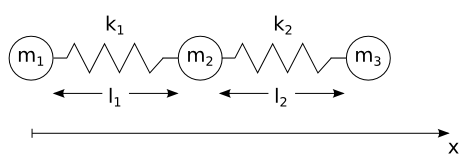
\includegraphics[width=0.8\textwidth]{images/3-masses-2-springs-linear.png}
\caption{Diagram for 3 masses attached with springs representing the nuclei motion.}
\label{fig:3-mases-2-springs}
\end{figure}

Considering the specific case for a O-Cu-O cluster, $m_1=m_3=m_O$, $m_2=m_{Cu}$ and $k_1=k_2\equiv k$, this model gives a symmetric and an antisymmetric frequencies (which we call \textit{Raman} and \textit{infrared} respectively) that depend on the masses: 

\begin{equation}\label{eq:omegaR}
\omega_{R}= \sqrt{k/m_O}
\end{equation}
\begin{equation}\label{eq:omegair}
\omega_{ir} = \sqrt{k(m_{Cu}+2m_O)/m_Om_{Cu}}
\end{equation}

Also, the coupling parameters depend on $m_O$\cite{?}:

\begin{equation}\label{eq:ir-coupl-isot}
\lambda_{ir}\propto (m_O\omega_{ir})^{-1/2}
\end{equation}
\begin{equation}\label{eq:Ram-coupl-isot}
\lambda_R\propto (m_O\omega_{R})^{-1/2}
\end{equation}

It can be seen from (\ref{eq:omegaR},\ref{eq:omegair},\ref{eq:ir-coupl-isot},\ref{eq:Ram-coupl-isot}) that a change, for example, $^{16}$O $\rightarrow$ $^{18}$O ammounts to a change in the frequencies  $\omega_{ir}$, $\omega_R$ and the couplings $\lambda_{ir}$ and $\lambda_R$. Taking the actual values for copper and oxygen, $m_{Cu}=63.546u$, $m_{^{16}O}=15.995u$ and $m_{^{18}O}=17.999u$ Isotopic change in the O-Cu-O cluster quantum model we obtain:

\begin{equation}\label{eq:omega-ir-isot}
\omega^{(16)}_{IR} / \omega^{(18)}_{IR} \simeq 1.039
\end{equation}
\begin{equation}\label{eq:lambda-ir-isot}
\lambda_R^{(16)} / \lambda_R^{(18)} \simeq 1.041
\end{equation}

In particular, the frequencies of the O-Cu-O cluster's two normal modes are given by (\ref{eq:omegaR},\ref{eq:omegair}). 
From here we identify the reduced masses:

\begin{equation}\label{eq:redMassR}
m_R = m_O \simeq 16.0\ u \simeq 2.6568 \times 10^{-26} kg
\end{equation}
\begin{equation}\label{eq:redMassIr}
m_{ir}=\frac{m_Om_{Cu}}{m_{Cu}+2m_O} \simeq 10.64\ u \simeq 1.7668 \times 10^{-26}kg
\end{equation}


\subsection{Isotopic shift for the excited states}

We define the relative isotopic shift for an excited state $i$ as 

\begin{equation}\label{eq:isot-shift-def-exc}
\Delta_i = \frac{E_i(^{16}O)- E_i(^{18}O)}{E_i(^{16}O)} \times 100
\end{equation}

where the energies $E_i$ are referred to the corresponding ground state.

\subsection{Isotopic shift for the ground state}

For the ground state we define the energy isotopic shift $\Delta_g$ in a similar way but with the energies measured relative to the uncoupled system Isotopic shift of polaron formation energy (that is, the system with $\lambda_{ir}=\lambda_R=0$).

\begin{equation}\label{eq:isot-shift-def-grd}
\Delta_g = \frac{\Delta E_g(^{16}O)- \Delta E_g(^{18}O)}{\Delta E_g(^{16}O)} \times 100
\end{equation}

where $\Delta E_g \equiv E_g - E_g(\lambda_{ir}=0, \lambda_R=0)$. To calculate this energies we need to take into account the \textit{zero-point energy} in (\ref{eq:phononic-part}) which should have been written as 

\begin{equation}\label{eq:phononic-part-complete}
H_{ph} = \hbar \omega_{ir} \left( a_{ir}^\dagger a_{ir} + \frac{1}{2}\right) + \hbar \omega_R\left( a_R^\dagger a_R + \frac{1}{2} \right)
\end{equation}


\section{Lattice distortions}

To understand the lattice distortion for excitations in the model hamiltonian (\ref{eq:full-hamiltonian}) it is useful to find the projection of a given state toreal space atomic coordinates. 
In a simple quantum harmonic oscillator with mass $m$ and frequency $\omega$ the creation and annihilation operators, $a^\dagger$ and $a$, are related to the real-space coordinate $x$ as

\begin{equation}\label{eq:harmOscRel}
x=\sqrt{\frac{\hbar}{2m\omega}}\left(a+a^\dagger\right)
\end{equation}

If we assume that phonon modes in our model hamiltonian (\ref{eq:phonon-part}) behave as quantum harmonic oscillators, we can define symmilar real space operators ($u_r,u_{ir}$) in terms of the bosonic creation and annihilation operatos ($b^\dagger,b$) for both, infrared and Raman, vibrational modes. 
These operators, called \textit{phonon coordinates}, are also related to the positions $x_i$ of the three sites in the cluster \cite{MustredeLeon1992},

\begin{equation}\label{eq:uR}
u_R \equiv \left(\frac{\hbar}{2 m_R \omega_R}\right)^{1/2}(b_R^\dagger + b_R) = \frac{x_3 - x_1}{\sqrt{2}}
\end{equation}

\begin{equation}\label{eq:uir}
u_{ir} \equiv \left(\frac{\hbar}{2 m_{ir} \omega_{ir}}\right)^{1/2}(b^\dagger_{ir}+b_{ir}) = \frac{ x_1 + x_3 - ( 2 m_O/m_{Cu})x_2}{(2 + 4 m_O/m_{Cu})^{1/2}}
\end{equation}

The reduced masses $m_R$ and $m_{ir}$ are determined in equations (\ref{eq:redMassR}-\ref{eq:redMassIr}).
In a quantum harmonic oscillator an energy eigenfunction, $\ket{n}$, has a projection into the real space coordinate $x$ given in terms of a Hermite polynomial of degree $n$, denoted by $H_n(x)$, in the following way,

\begin{equation}\label{eq:harmOscProj}
\braket{x}{n} 
\equiv \psi_n(x) 
= \frac{1}{\sqrt{2^n n!}} \left(\frac{m \omega}{\pi \hbar}\right)^{1/4}
  \exp\left(-\frac{m \omega x^2}{2 \hbar}\right) H_n\left( \sqrt{\frac{m \omega}{\hbar}} x \right) 
\end{equation}


For an arbitrary wavefunction $\ket{\psi} = \sum_n \braket{n}{\psi} \ket{n}$ the projection in real space is $\braket{x}{\psi} = \sum_n \braket{n}{\psi} \braket{x}{n}$ with $\braket{x}{n}$ given by \ref{eq:harmOscProj}.

For the model hamiltonian \ref{eq:full-hamiltonian}, as discussed in section \ref{sec:basis-set}, a possible basis set is given by the functions ${| e_1, e_2, ir, R \rangle}$ with $e_i$ the position of the $i$-th electron and $ir$, $R$ the number of infrared and Raman phonons respectively. 
Thus an arbitrary wavefunction in this system, $\ket{\psi}$, can be expanded as

\begin{equation}\label{eq:wf-phonon-base}
\ket{\psi}=\sum_{e_1,e_2,ir,R} \braket{e_1,e_2,ir,R}{\psi}\ket{e_1,e_2,ir,R}
\end{equation}

\noindent and we can make the partial projection into the phonon coordinates $(u_{ir},u_R)$ as defined by (\ref{eq:uR},\ref{eq:uir})

\begin{equation}\label{eq:wf-expansion}
\braket{u_{ir},u_R}{\psi}=\sum_{e_1,e_2,ir,R} \braket{e_1,e_2,ir,R}{\psi}\braket{u_{ir},u_R}{ir,R}\ket{e_1,e_2}
\end{equation}

\noindent where we have denoted $\braket{u_{ir},u_r}{e_1,e_2,ir,R}=\braket{u_{ir},u_R}{ir,R}\ket{e_1,e_2}$. 
The term $\braket{u_{ir},u_r}{ir,R}$ is similar to (\ref{eq:harmOscProj}) but considering both phonon modes:

\begin{equation}\label{eq:hermite-expansion}
\braket{u_{ir},u_r}{ir,R}  = \frac{\left(m_{ir}m_R\right)^{1/4}}{\sqrt{2^{(ir+R)} ir!R!\pi\hbar}}
\exp\left(-\frac{\tilde{u}_{ir}^2 + \tilde{u}_R^2}{2}\right) 
H_{ir}\left(\tilde{u}_{ir} \right)H_{R}\left(\tilde{u}_{R} \right)
\end{equation}

\noindent where we have defined,

\begin{equation}\label{eq:uTildeDef}
\tilde{u}_j \equiv \sqrt{\frac{m_j\omega_x}{\hbar}}\ u_j
\end{equation}

\noindent for $j=ir,R$. 
Now, from (\ref{eq:wf-expansion}), the probability amplitude of findind a state $\ket{\psi}$ proyected into phonon coordinates $(u_{ir},u_R)$ for a given site occupation $(e_1,e_2)$ is

\begin{equation}
\begin{split}
& \left|\braket{e_1,e_2,ir,R}{\psi}\right|^2 \\
& \ \ = \left|\sum_{e_1',e_2',ir,R}\braket{e_1,e_2,ir,R}{\psi}\braket{u_{ir},u_R}{ir,R}\braket{e_1,e_2}{e_1',e_2'}\right|^2 \\
& \ \ = \left|\sum_{ir,R}\braket{e_1,e_2,ir,R}{\psi}\braket{u_{ir},u_R}{ir,R}\right|^2
\end{split}
\end{equation}

Finally, the probability amplitude of finding a system in the state $\ket\psi$ with phonon coordinates ($u_{ir},u_R$) irrespective of the electronic configuration is given by the sum over the electronic degrees of freedom on the previous equation,

\begin{equation}\label{eq:phonon-coord-projection}
\begin{split} \left|\psi(u_{ir}, u_R)\right|^2 & \equiv \sum_{e_1,e_2}\left|\braket{e_1,e_2,ir,R}{\psi}\right|^2 \\
& = \sum_{e_1,e_2} \left|\sum_{ir,R}\braket{e_1,e_2,ir,R}{\psi}\braket{u_{ir},u_R}{ir,R}\right|^2
\end{split}
\end{equation}

\noindent with $\braket{u_{ir},u_R}{ir,R}$ given by (\ref{eq:hermite-expansion}).

The projection \ref{eq:phonon-coord-projection} allows us to calculate the probability amplitude of finding a specific distortion in the atomic coordinates for the O-Cu-O cluster.
With the atomic coordinates $x_i$, as defined in section \ref{sec:isotopic-model}, the difference $d$ in O-Cu bond lengths is

\begin{equation}\label{eq:bondDiff}
d= \left| (x_3 - x_2) - (x_2 - x_1) \right| = \left| x_1 + x_3 - 2x_2 \right|
\end{equation}

The $x_i$ coordinates are varying at all times but taking an instant in which $x_2=0$ we can simplify (\ref{eq:bondDiff}) to

\begin{equation}\label{eq:bondDiffSimpl}
d=\left|x_1+x_3\right|
\end{equation}

And, from $u_{ir}$'s definition in (\ref{eq:uir}),

\begin{equation}\label{eq:uirSimpl}
u_{ir}=\frac{x_1+x_3}{\left( 2+4 m_O/m_{Cu} \right)^{1/2}}
\end{equation}

Now using (\ref{eq:bondDiffSimpl}) and (\ref{eq:uirSimpl}) gives us

\begin{equation}\label{eq:uirvsd}
\left|u_{ir}\right|=\frac{d}{\left( 2+4 m_O/m_{Cu} \right)^{1/2}}
\end{equation}

or, solving for $d$,

\begin{equation}\label{eq:dvsuir}
d=\sqrt{2}\left(1 + 2\frac{m_O}{m_{Cu}} \right)^{1/2}\left|u_{ir}\right|
\end{equation}

which is a relationship between the phonon coordinates, wich can be calculated from the model's eigenfunctions and the observable lattice distortion.

\section{Projection into states with definite electron occupation numbers}

Eigenstates of the hamltonian \ref{eq:full-hamiltonian} have delocalized charges.
To understand charge dynamics according for each excitation it is useful to project the eigenstates into the definite electron occupation basis states discussed in section \ref{sec:basis-set} by summing over phononic degrees of freedom.
That is, for a given eigenstate $\ket{\psi}$ we can find its probability of having its first hole in site $e_1$ and the second on site $e_2$ (with $e_1$, $e_2=1,2,3$) by making the projection

\begin{equation}\label{eq:electron-occupation}
\braket{e_2,e_2}{\psi} = \sum_{i=0}^{N_{ir}}\sum_{R=0}^{N_R} \braket{e_1,e_2,i,R}{\psi}
\end{equation}

\section{Choice of parameters}

To choose values for this model we take representative values guided from local-density approximations \cite{Pickett1989}. 
In particular Ref. \cite{DeWeert1989}, using a tight-binding model, reports a band energy of $E_0$ = 0.35 eV and a hopping parameter of $t=0.43-0.74$ eV, for Cu(1)-O(4) sites.
The on-site Coulomb repulsion in La$_2$CuO$_4$, $U$  is estimated to be in the range $4.0-10.5$ eV, \cite{Hybertsen1989}. 

The bare phonon frequencies are fixed to values found experimentally in optical and inelastic neutron scattering experiments $\omega_R = 500\ cm^{-1}$ and $\omega_{ir} = 612.4\ cm^{-1}$ for YBa$_2$Cu$_3$O$_7$ \cite{?}.

In order to consider the simplest possible model we make the further assumption of taking the on-site Coulomb repulsion in the copper and oxygen sites to be equal with no nearest neighbor Coulomb repulsion. 
We also use a single hopping parameter $t$ and ignore hopping between the two oxygen sites. 
Since only the coupling between the asymmetric mode and the charge motion leads to a measurable lattice distortion, with two Cu–O bond lengths, we only consider the effect of the variation in the electron–lattice coupling constant with the antisymmetric mode, $\lambda_{ir}$, and we set the electron-lattice coupling with the symmetric mode, $\lambda_R$ , as zero \cite{Salkola1995}. 
The inclusion of those considerations in the model, or other choices of parameters (e.g. \cite{Salkola1994, Salkola1995}) yield very similar results.
The relevant value for the coupling $\lambda_{ir}$ is determined using equation \ref{eq:dvsuir}; it is chosen such that the ground state has a maximum probability density at a $u_{ir}$ that reproduces the observed lattice distortion of 0.13 \AA \cite{?}.
In this work we use the same parameters as \cite{Mena2006, DeLeon1999, Leon2008, MirandaMena2007}:

\begin{itemize}
\item On-site Coulomb repulsion for O(4) and Cu(1) sites: $U=7$ eV
\item Nearest-neighbor hopping: $t=0.5$ eV
\item Band energy for O(4) and Cu(1) sites: $E_0=0.5$ eV
\item Bare phonon frequency for the Raman mode: $\omega_R=500$ cm$^{-1}$
\item Bare phonon frequency for the infrared mode: $\omega_{ir}=612.4$ cm$^{-1}$
\end{itemize}

These are the parameters used for this model in other publications\footnote{It seems that the reported values for the phonon frequencies in \cite{Salkola1994, Salkola1995} are erroneous since they show $\omega_R > \omega_{ir}$ and they are inconsistent from what can be observed in Fig. 1 of \cite{Salkola1994} at $\lambda_{IR}=0$.}.

\noindent\begin{tabular}{| l | c | c | c | c | c |}
\hline
Reference & $U$ (eV) & $\epsilon$ (eV) & $t$ (eV) & $\omega_{ir}$ (cm$^{-1}$) & $\omega_R$(cm$^{-1)}$ \\
\hline
\cite{MustredeLeon1992} & 7.0 & 0.5 & 0.5 & 600 & 500 \\ 
\cite{Salkola1994, Salkola1995} & 4.44 & 0.307 & 0.634 & 477.7 & 576  \\
\cite{Mena2006,DeLeon1999, Leon2008, MirandaMena2007} & 7.0 & 0.5 & 0.5 & 612.4 & 500 \\ 
\cite{MustredeLeon2000} & 4.44 & 0.307 & 0.634 & 600 & 500 \\
\hline
\end{tabular}

\section{Classification of the excitations}
\label{sec:classification}

% - We can't separate the eigenstates as products of electronic and phononic parts
% - Dispersions are small (plot?) so we can still identify them as "electronic" or "phononic"
% - Following the eigenvalue, mean ir (Ram) and their dispersions we can track them with increasing couling (plot?)
% Maybe include the plot projecting the electronic state at \lambda_{ir}>0 with itself at \lambda_{ir}=0

As previously noted, for electron-lattice coupling values $(\lambda_{ir},\lambda_R)$ different from zero, the eigenstates of the many-body Hamiltonian (\ref{eq:full-hamiltonian}) cannot be described as a direct product of purely electronic and phononic states. 
This would correspond to the usual adiabatic method (Born-Oppenheimer approximation) allowing a separation of ionic and electronic motion $\psi_{elec}\psi_{phononic}$. 
In our case the total wave function describing the ground state or its excitations is a linear combination of states which are separate products of the electronic and phononic wave functions. 
However, for the electron-lattice coupling range we are considering, the mean-phonons' dispersions remain small and the identification of some states as electronic-like or lattice-like in esence remains a useful interpretation.


\section{Computational details}
\label{sec:comp_details}

% Size of the base
% Convergence
% Computational resources

We performed an exact diagonalization of the Hamiltonian matrix with a basis of 8649 states using a QR algorithm \cite{eigenweb}. 
The basis includes states of two holes on the three sites, 30 harmonic Raman phonons and 30 harmonic infrared phonons. 
Since we are performing a diagonalization of the full Hamiltonian matrix our results do not rely in approximations such as the adiabatic or the anti-adiabatic approximations. 
The  truncation of the basis to 30 phonons of each kind could introduce innacuracies, however we found this choice to be an adecuate description for the few lowest energy states we are considering up to electron-lattice couplings ~0.25 eV (see figure 3).
